\chapter{\label{chap:intro}Metodologia de Pesquisa}

A metodologia de pesquisa escolhida para este trabalho, é composta de um revisão da literatura já elaborada por Steglich e colegas \cite{caio2019} e de uma \textit{survey} que ainda será realizada. Para Kitchenham end Pfleeger \cite{pfleeger2001principles} uma \textit{survey} consiste em sistema de coleta de dados e informações objetivando decifrar conhecimentos e práticas adotadas pelos sujeitos da pesquisa.
   
As etapas que compõe uma pesquisa \textit{survey} são:  definição do objetivo da pesquisa, definição da população e da amostra, elaboração do questionário, coleta de dados, processamento dos dados, análise dos dados e divulgação dos resultados \cite{vieira2010dicionario}.

\begin{figure}
    \centering
    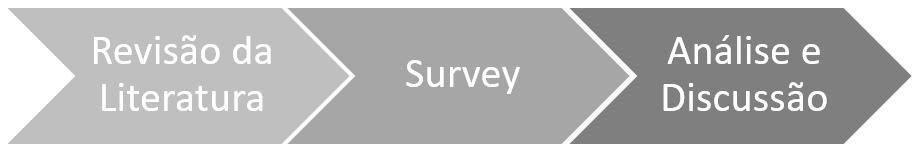
\includegraphics[scale=0.66]{fig/metodologia.PNG}
    \caption{Metodologia de Pesquisa}
    \label{fig:my_label}
\end{figure}


\section{\textbf{Revisão da Literatura e Definição do Escopo}}

%Pretendeu-se aprofundar o conhecimento na literatura de segurança em Ecossistemas de Software Móvel(ECOSM) e também em controles presentes na ISO 27002 utilizando como base a revisão da literatura feita por Steglich e colegas \cite{caio2019} que teve como objetivo identificar quais controles da ISO 27001 estão presentes na literatura de ECOSM, buscando verificar evidências sobre como eles são usados e o que a literatura relata sobre esses controles. O resultado do estudo mostrou que apenas 34 dos 114 controles da ISO 27001 estavam presentes na literatura de ECOSM e que apenas 2 de um total de 14 seções tinham seus respectivos controles evidenciados na literatura de ECOSM . Essas seções são, políticas de segurança da informação e criptografia. A falta de literatura sobre a maioria dos controles da ISO 27002, motivou o desenvolvimento deste trabalho.

 Com o objetivo de entender a  ISO 27002 e identificar quais os controles dela estão presentes na literatura,
 utilizou-se a revisão da literatura de Steglich e colegas \cite{caio2019}. Restringiu-se a literatura ao artigo citado, dado que o mesmo consolida toda  a literatura na área. O artigo é uma revisão de autoria do orientador desde TCC, realizada em 2019, quando este trabalho se iniciou. Este artigo teve como objetivo identificar quais controles da ISO 27001 estão presentes na literatura de ECOSM, buscando verificar evidências sobre como eles são usados e o que a literatura relata sobre esses controles. O resultado do estudo mostrou que apenas 34 dos 114 controles da ISO 27001 estavam presentes na literatura de ECOSM e que apenas 2 de um total de 14 seções tinham seus respectivos controles evidenciados na literatura de ECOSM . Essas seções são, políticas de segurança da informação e criptografia. A falta de literatura sobre a maioria dos controles da ISO 27002, motivou o desenvolvimento deste trabalho, que ocorreu da seguinte forma:
 
 \begin{itemize}
    \item Passo 1: Primeiramente realizou-se um estudo em profundidade com o objetivo de entender a ISO 27002 e seus controles.
   
    \item Passo 2: Identificação de quais seções presentes na ISO 27002 estava de acordo com proposta deste TCC.
    
     \item Passo 3: Reuniões para a decisão e deliberação de quais seções seriam mantidas e retiradas por estarem fora do escopo do trabalho.
      
    \item Passo 4: Revisão com um especialista, das seções da ISO 27002 que foram selecionadas.
  \end{itemize}

 
 %A partir da identificação de quais seções da ISO 27002 estavam de acordo com a proposta, e do estudo...
 \noindent \paragraph{\textbf{Passo 1:} A partir do estudo de Steglich e colegas \cite{caio2019} e do estudo aprofundado de quais seções da ISO 27002 estavam de acordo com a proposta, foi possível aprofundar o conhecimento sobre as normas e sua relevância para este trabalho.}
 
 \noindent \paragraph{\textbf{Passo 2:} Inicialmente começou-se interpretando as seções e seus controles verificando a complexidade de cada uma no contexto de ecossistema de software móvel. Na primeira seleção das seção alguns controles e objetivos de controle foram retirados por não estarem relacionados com desenvolvimento de de software}
 
 \noindent 
    \paragraph{
    \textbf{Passo 3:} Para aprimorar a filtragem realizada inicialmente, foram realizadas discussões com 3 pesquisadores, com experiência nas áreas de auditoria, metodologia de pesquisa e ecossistemas de software móvel. Foram feitas reuniões de uma hora, conduzidas pelo autor deste trabalho e com isso foi possível eliminar as seções irrelevantes e manter outras.
    }
 
    \paragraph{
  A partir da filtragem de seções e controles com os pesquisadores, foi possível eliminar as Seções 5, 6, 7, 8, 11, 13, 15, 16, 17, 18 pois seus controles e objetivos de controle não se enquadravam no objetivo deste TCC, que  pretende ter como foco controles que se enquadrem no desenvolvimento de software mobile. Por exemplo, a Seção 7 trata Segurança dos Recursos Humanos. No entendimento do autor deste TCC e em alinhamento com os três pesquisadores que participaram das discussões nessa etapa inicial, entendeu-se que a Seção está fora do escopo de desenvolvimento de software, pois trata de como evitar o vazamento de informações por colaboradores.\todo{XXXX} Detalhes podem ser consultados no apêndice B. %Nas Figuras 5.5, 5.6, 5.7, 5.8, 5.9, 5.10, 5.11, 5.12, 5.13 e 5.14 podem ser encontradas as seções retiradas na filtragem. 
  As Seções 9, 10, 12, 14 foram mantidas e alguns de seus objetivos de controle retirados devido a análise conjunta dos pesquisadores durante a discussão. Após a filtragem das seções com os 3 pesquisadores, convidamos um especialista convidamos um especialista, com o intuito de validar o escopo das seções e das peguntas elaboradas. \todo[inline]{como falar do apêndice?} 
    }
    
  \noindent
    \paragraph{
    \textbf{Passo 4:} Visando confirmar a relevância dos controles selecionados, presentes na ISO/IEC 27002, buscou-se estratégias para que de fato os controles selecionados fossem relevantes para a execução de uma \textit{survey} com desenvolvedores de software móveis. Para isso, usou-se a abordagem de Entrevista com Especialistas para avaliação dos controles selecionados previamente, conforme recomendado por Flick \cite{flick2018introduction}. O autor esclarece que entrevistar especialistas pode servir a três propósitos: i) para exploração, para orientação em um novo campo, a fim de auxiliar a geração de hipóteses; ii) pode ser usada para coletar informações de contexto complementando percepções provenientes da aplicação de outros métodos; ou iii) pode também ser usada para geração de teorias que visam desenvolver uma tipologia ou uma teoria sobre uma questão a partir da reconstrução do conhecimento de vários especialistas. Com base no que foi expressado pelo autor \cite{flick2018introduction}, as entrevistas com os especialistas sarão utilizadas com o propósito ii), de coletar informações com a finalidade de complementar as percepções a respeito dos controles presentes na ISO/IEC 27002 que foram selecionados previamente e revisar a sua relevância.
    }
    
    \paragraph{
    Foi convidado, por conveniência, um especialista para participar desta avaliação, após a filtragem com os três pesquisadores para selecionar os controles presentes na ISO/IEC 27002, que fossem direcionados para a área da computação e elaborar perguntas referentes a cada controle da ISO/IEC 27002. Para que as perguntas sejam utilizadas na elaboração de um questionário com diversos desenvolvedores. O perfil deste especialista é como segue:}   
    
    \paragraph{
    O entrevistado é de Alvorada, RS, cidade da região metropolitana de Porto Alegre, já tendo atuado em outros países em projetos de tecnologias móveis, sendo desenvolvedor da área há 12 anos e atualmente como instrutor. Ao longo destes 12 anos, este especialista colaborou com os ECOS Android, iOS, WindowsPhone e Blackberry.
    }
    
    \paragraph{
    A partir da entrevista com o especialista foi possível verificar se as perguntas condiziam com preocupações ou atividades de um desenvolvedor de aplicações móveis. Nesta revisão ficou resolvido que o a maioria das perguntas estavam adequadas com o tema proposto e foram sugeridas as remoções de 21 perguntas de um total de 78.}
    
    %\todo[inline]{ Posteriormente a entrevista com o especialista, 3 pesquisadores da área de ES reconheceram outro conjunto de perguntas que poderiam ser removidas, pois condiziam com elementos de gestão organizacional e não de TI ou desenvolvimento de software.(ESSA PARTE ESTÁ ADEQUADA?)}
    
 

 
 

 

 
 %Nas figuras 5.1, 5.2, 5.3 e 5.4 estão representados os controles mantidos \todo[inline]{citar apendice ? e onde fica melhor de colocar essa frase? "nas figuras..."}
 
 %e serão validadas futuramente com um especialista numa entrevista, para que assim seja possível elaborar a survey e dar continuidade as etapas da metodologia de pesquisa do trabalho.  
 
 
 
 






\section{\textbf{\textit{Survey}}} Definiu-se como objetivo de pesquisa, conhecer quais os controles da ISO 27002 são adotados por desenvolvedores de software mobile e quais são as dificuldades enfrentadas ao tentar adotá-los, além de propor recomendações de como sobrepor essas dificuldades.Para atingir o objetivo do trabalho os seguintes passos foram realizados:
\begin{itemize}

\item \textbf{Construir instrumento de coleta:} Para elaborar o questionário serão considerados os resultados anteriores das entrevistas com especialistas. O perfil desejado para a realização da pesquisa será de desenvolvedores de software mobile. A partir da revisão de escopo com 

\item \textbf{Validação do instrumento de coleta:} O instrumento foi validado com dois participantes. O primeiro participante é de Manaus, AM, sendo professor e pesquisador com 10 anos de experiência na área, sendo 2 anos como desenvolvedor de aplicações, 4 anos como evangelista de desenvolvedores e 4 anos como pesquisador da área. Já colaborou nos ECOS Android, Windows Phone, Nokia e Symbian. Com este participante foi possível  melhorar o entendimento de algumas perguntas, com o intuito de deixar-las mais claras, além de ter uma estimativa do tempo de 20 minutos de resposta do questionário. O segundo participante é professor no Instituto Federal do Rio Grande do Sul e tem 3 anos de pesquisa com empresas em desenvolvimento mobile. Com este participante foi possível avaliar o conteúdo técnico de algumas perguntas para que os futuros respondentes não tivessem dúvidas ao responder o questionário.


%O questionários será validado com desenvolvedores mobile com experiência alguns anos de experiência. Será realizado um piloto do questionário com colegas de curso que entendem de desenvolvimento mobile

 \textbf{Piloto:} Também como parte da validação do instrumento, realizou-se o piloto com o objetivo identificar qualquer prolema com o questionário, antes da coleta da coleta dos dados. Este piloto foi realizado com 2 participantes. 
 
 O primeiro participante é estudante de Engenharia de Software na Pontifícia Universidade Católica do Rio Grande do Sul e participou do programa de capacitação Apple Developer Academy. O participante levou  14 minutos para responder a \textit{survey} e considerou que o fluxo nas das questões estavam bem estruturadas, sem a necessidade de alguma alteração.
 
 O segundo participante é estudante de ciência da computação na PUCRS e trabalha como \textit{quality assurance}. O participante levou 16 minutos para responder a \textit{survey} e verificou alguns erros de formatação no texto, que foram corrigidos posteriormente.  
 

\item \textbf{Coleta dos Dados:} A coleta foi realizada somente de maneira online pelas limitações da pandemia. Inicialmente o instrumento foi divulgado no LinkedIn com o objetivo de atingir a rede de contatos que se enquadravam no perfil desejado de desenvolvedores mobile. O instrumento também foi divulgado em grupos de desenvolvedores iOS e Android no Slack e Facebook. 

Devido a baixa taxa de respondentes entrou-se em contato individualmente com desenvolvedores de dispositivos móveis presentes na rede de contatos do LinkedIn, com o objetivo de obter mais respostas. Os pesquisadores que auxiliaram na separação das seções da ISO 27002 também auxiliaram na divulgação da \textit{survey} , divulgando-a para sua rede de contatos. 


\todo[inline]{como ficou?}
\item \textbf{Analisar resultados:} Com o resultado do questionário foi realizada a análise dos dados, que pode ser consultada no Capítulo 5. Separou-se cada questão individualmente, observando se o seu resultado demonstrava ou não uma preocupação dos desenvolvedores.
\end{itemize}

%\todo[inline]{Tiro tudo isso aqui, certo? virou projeto futuro} 
%\section{\textbf{Definição do Guia de Recomendações}}

%Requisitos de segurança como confidencialidade, integridade são abstratos e suas aplicações necessitam de uma orientação para serem seguidos, para que seja possível atender aos requisitos. Com os resultados da \textit{survey} ira ser criado um guia de recomendações de boas práticas com objetivo de auxiliar desenvolvedores a adotarem os controles previstos na ISO 27002. 

%No processo para a elaboração do guia de recomendações pretende-se desenvolver um critério para a categorização de cada uma das orientações. O principal objetivo por trás dessa classificação é preparar a base para expressar esses guias em uma linguagem formal e argumentar sobre sua satisfação \cite{zhioua2016security}.


